\chapter{Project organisatie} \label{chap:ProjectOrganisatie}
\section{Externe interfaces}
Dit project wordt geproduceerd in opdracht van het vak Software Engineering. Communicatie verloopt via mail met Jens Nicolay\footnote{\href{mailto:jnicolay@vub.ac.be}{jnicolay@vub.ac.be}}, Ragnild van Der Straeten\footnote{\href{mailto:rvdstrae@vub.ac.be}{rvdstrae@vub.ac.be}} en Dirk van Deun\footnote{\href{mailto:dirk@dinf.vub.ac.be}{dirk@dinf.vub.ac.be}}. Jens Nicolay en Ragnild van Der Straeten worden gecontacteerd voor functionale zaken, terwijl Dirk van Deun gecontacteerd wordt voor technische zaken betreffende de infrastructuur.

\section{Interne structuur} \label{sec:InterneStructuur}
Voor dit project is er een team van 7 personen. De takenverdeling binnen dit team is als volgt:
\begin{table} [H]
	\centering
	\caption{Takenverdeling.}
	\begin{tabular} {l|cc}
		Rol & Verantwoordelijke & Reserve \\
		\hline
		Project Manager & Pieter & Nicolas \\
		Configuration Manager & Christophe & Tim \\
		Database Manager & Nicolas & Christophe \\
		Quality assurance Manager & Sam & Youri \\
		Requirements Manager & Fernando & Pieter \\
		Design Manager & Youri & Sam \\
		Implementation Manager & Tim & Fernando \\
		\hline
		Webmaster & Christophe & \textbackslash \\
		Secretaris & Fernando & \textbackslash 
	\end{tabular}
	\label{tab:takenverdeling}
\end{table}

Communicatie binnen het team verloopt via de website \cite{portalWebsite}. Hier wordt een soort blog gebruikt door de teamleden. Een teamlid kan een bericht plaatsen en achteraf kan op dit bericht gereageerd worden door andere teamleden. Een voorbeeldinteractie is weergegeven in figuur \ref{fig:communicatieExample}. Verder wordt er gebruik gemaakt van de mailinglijst op wilma om de verschillende teamleden van een notificatie te voorzien bij de aanmaak van een nieuw bericht. 
\begin{figure} [H]
	\centering
	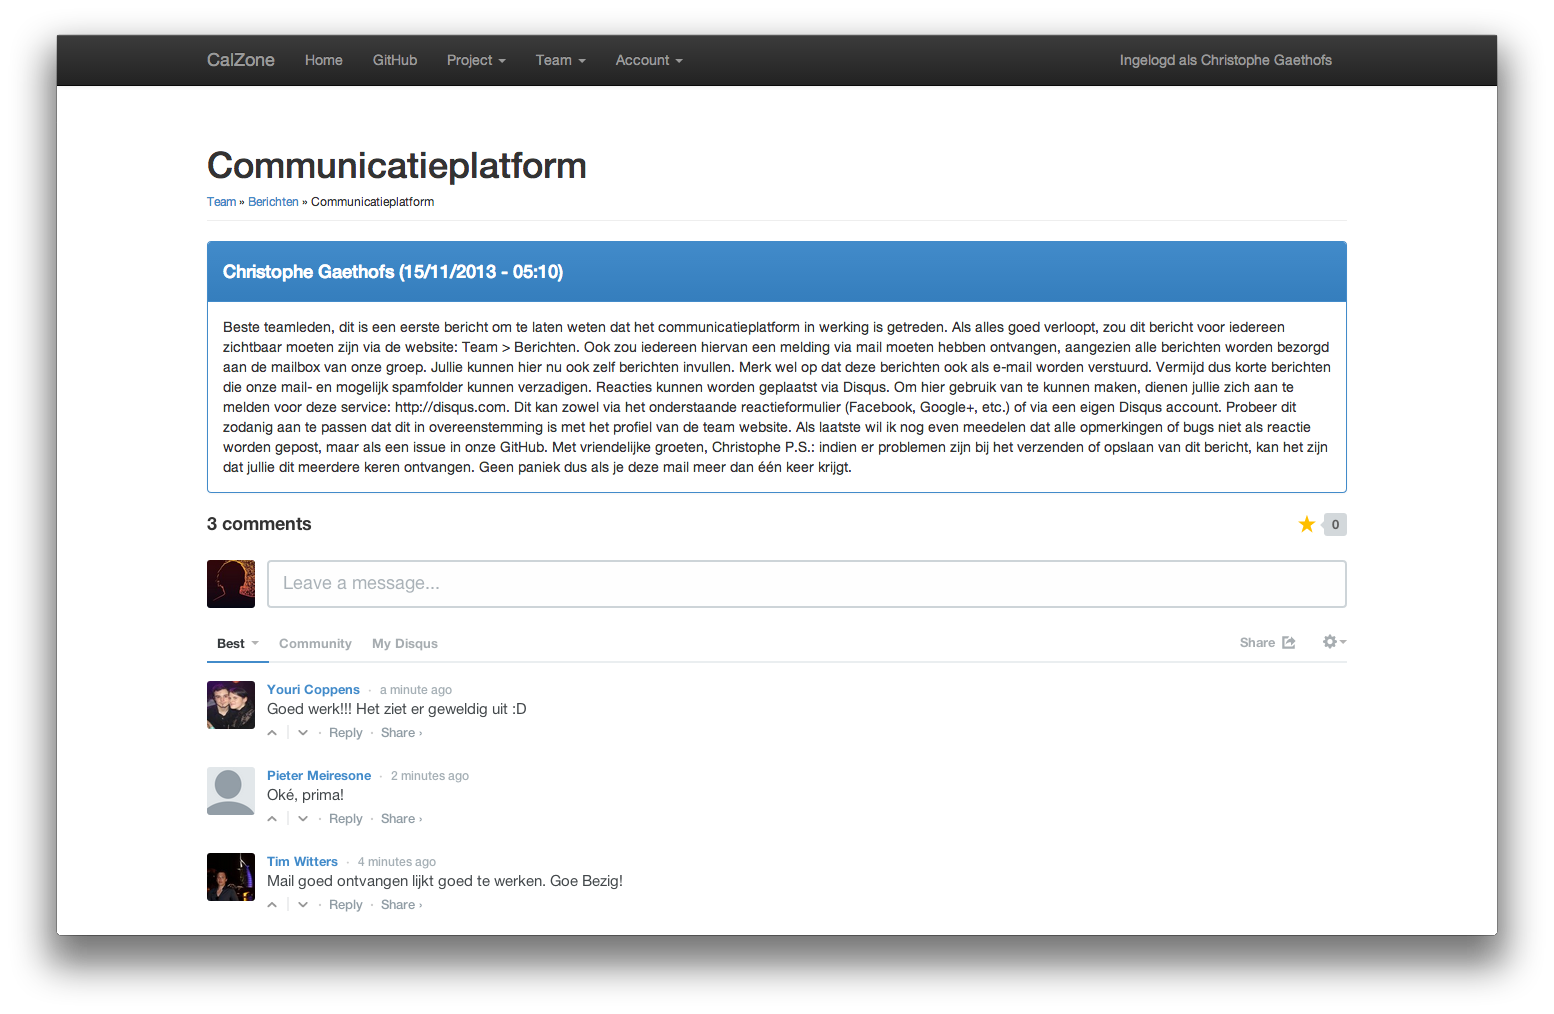
\includegraphics[width = \textwidth]{ProjectOrganization/Communication.png}
	\caption{Communicatie op de team website.}
	\label{fig:communicatieExample}
\end{figure}

\section{Rollen en verantwoordelijkheden}
Elk teamlid is verantwoordelijk voor een functie en reserve van een andere functie (zie tabel \ref{tab:takenverdeling}).Ook speelt elk teamlid een rol in de codering van het systeem. 

Hier volgt een gedetailleerd overzicht van deze functies:
\begin{table} [H]
	\centering
	\caption{Functies.}
	\begin{tabular} {l | p{10cm}}
		Functie & Verantwoordelijkheden \\
		\hline
		Project Manager &  
		\begin{itemize}
		\item Verantwoordelijkheid over SPMP
		\item Opvolging van managers
		\item Zorgt ervoor dat deadlines binnen het team gerespecteerd worden
		\item Ingrijpen waar nodig
		\end{itemize}\\
		\hline
		Configuration Manager &
		\begin{itemize}
		\item Verantwoordelijkheid over SCMP (onderdeel van SPMP)
		\item Keuze software en procedures
		\item Controle van gebruik van software en instellingen.
		\end{itemize}\\
		\hline
		Database Manager &
		\begin{itemize}
		\item Onderhoud en controle database
		\item Onderscheid maken tussen en beheren van test en officiële database
		\end{itemize}\\
		\hline
		Quality Assurance Manager &
		\begin{itemize}
		\item Verantwoordelijkheid over SQAP (onderdeel van SPMP)
		\item Verantwoordelijkheid over STD
		\item Controle en correctie van nauwkeurigheid en styling van code en documenten
		\item Toezien op de uitvoering van testen.
		\end{itemize}\\
		\hline
		Requirements Manager &
		\begin{itemize}
		\item Verantwoordelijkheid over SRS
		\item Controle van uitvoering van requirements
		\item Verificatie van uitgewerkte requirements
		\end{itemize}\\
		\hline
		Design Manager &
		\begin{itemize}
		\item Verantwoordelijkheid over SDD
		\item modelleren en architectuur bepalen van het systeem
		\end{itemize}
	\end{tabular}
	\label{tab:functies}
\end{table}
\begin{table} [H]
	\centering
	\caption{Functies (vervolg).}
	\begin{tabular} {l | p{10cm}}
		Functie & Verantwoordelijkheden \\
		\hline
		Implementation Manager &
		\begin{itemize}
		\item Verdelen van system requirements onder de developers
		\item Controle van de progressie van de code
		\item Controle van de uitvoering van het design
		\end{itemize}\\
		\hline
		Webmaster &
		\begin{itemize}
		\item Onderhoud teamwebsite
		\item Onderhoud projectwebsite (die dat de gebruikers van het systeem gebruiken).
		\end{itemize}\\
		\hline
		Secretaris &
		\begin{itemize}
		\item Verslagen van vergaderingen bijhouden
		\end{itemize}\\
	\end{tabular}
\end{table}